% Provenance (never printed): the food, energy and environment strand of ../economics_series.md;
% water from the geography programme (one paragraph). Brief: sources/book1/BRIEFS.md, g6-06.
% Chart data: figdata/grade-6/06-food-and-energy (FAOSTAT crops; WDI EG.USE.PCAP.KG.OE,
% NY.GDP.PCAP.PP.KD, SP.POP.TOTL, ER.H2O.FWTL.ZS; BLS Consumer Expenditure Surveys 2025;
% CEDS SO2 and CO2; Brenland household survey).
\chapter{Food and Energy}\label{ch:g6:food-and-energy}

Every person needs food every day, and every machine, lamp and stove needs
energy. Two centuries ago, most families spent most of their income on food,
and most of their energy came from wood, animals and their own muscles. This
chapter follows how much grain a field gives, how much of a budget goes to food,
how much energy people use --- and the smoke that came with it.

\begin{omfigure}
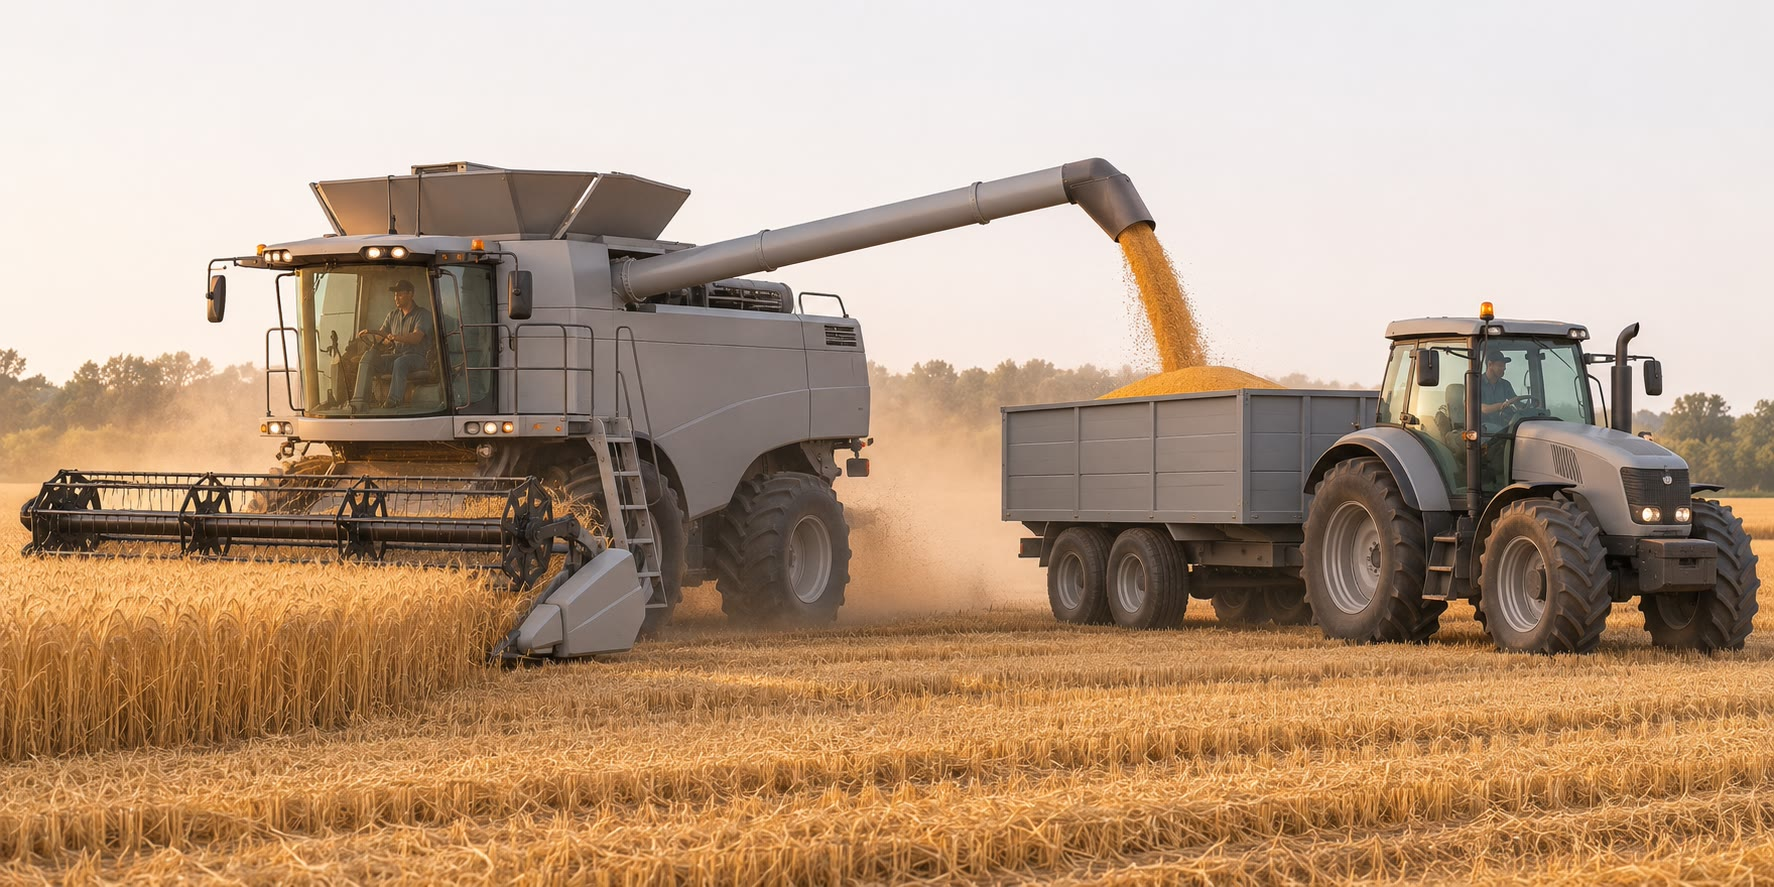
\includegraphics[width=0.62\linewidth]{images/book1/ai/g6-food-and-energy-harvest-plain.jpg}

{\small Harvesting wheat with a combine harvester. One machine now does the
work that once needed dozens of people with sickles.}
\end{omfigure}

\begin{recall}
\omterm{def:g6:reading-economic-charts:per-person}{Per-person values} and the \omterm{def:g6:reading-economic-charts:times-ten-scale}{times-ten scale} were defined in
\cref{ch:g6:reading-economic-charts}, \omterm{def:g6:living-standards:income-per-person}{income per person} in
\cref{ch:g6:living-standards}.
\end{recall}

\section{More grain from each field}

\begin{definition}[Crop yield]\label{def:g6:food-and-energy:crop-yield}
The \emph{yield}\index{crop yield} of a crop is the quantity harvested from
one hectare of land in one year (a hectare is a square of 100 metres by
100 metres):
\[
  \text{yield} = \frac{\text{quantity harvested}}{\text{area harvested}}.
\]
\end{definition}

\begin{measure}[Yield]
Statistical offices estimate the harvest of each crop from farm surveys, sales
records and, more and more, satellite pictures of the fields, and they measure
the area that was harvested. The Food and Agriculture Organization of the United
Nations collects these numbers from almost every country and adds them up by
region. ``Cereals'' are wheat, rice, maize, barley and the other grains.
\end{measure}

\begin{omchart}{Cereal yields, 1961--2024, in tonnes of grain per hectare
harvested, in five regions and the world.}{Food and Agriculture Organization of
the United Nations, FAOSTAT, crops: cereals, primary, \omterm{def:g6:food-and-energy:crop-yield}{yield}}
\begin{tikzpicture}
\begin{axis}[omtime, xmin=1961, xmax=2024, ymin=0, ymax=8,
  xtick={1965,1975,1985,1995,2005,2015}, xlabel={Year},
  ylabel={Tonnes per hectare}, height=0.56\linewidth,
  legend style={at={(0.5,-0.2)}, anchor=north, legend columns=3},
  cycle list={{black, thick, densely dashed}, {omThm, thick}, {omExo, thick},
    {omProp, thick}, {omDef, thick}, {omMeth, thick}}]
\pgfplotsforeachungrouped \col in {world, africa, asia, europe, n_america, s_america} {
  \addplot table[x=year, y=\col] {figdata/grade-6/06-food-and-energy/out/cereal_yields.csv};
}
\legend{World, Africa, Asia, Europe, Northern America, South America}
\end{axis}
\end{tikzpicture}
\end{omchart}

% figdata: cereal_yields (world 1961 1.35, 2024 4.21; africa 1961 0.81, 2024 1.68;
% n_america 1961 2.20, 2024 7.42)
In 1961, a hectare of cereals gave $1.35$ tonnes of grain on average in the
world; in 2024, $4.21$ tonnes, more than three times as much. New varieties of
seeds, fertilisers, irrigation and machines did it. The rise was very unequal:
in Northern America, from $2.20$ to $7.42$ tonnes; in Africa, from $0.81$ to
$1.68$ tonnes. Because \omterm{def:g6:food-and-energy:crop-yield}{yields} rose faster than the population, the world
produces more grain per person than in 1961.

\section{Famine}

\begin{definition}[Famine]\label{def:g6:food-and-energy:famine}
A \emph{famine}\index{famine} is a time when so many people in a region cannot
get enough food that many of them die of hunger or of the diseases that hunger
brings.
\end{definition}

\omterm{def:g6:food-and-energy:famine}{Famines} were common for most of history. In the 1800s and 1900s, the largest
\omterm{def:g6:food-and-energy:famine}{famines} killed millions of people each, in Ireland, India, China, the Soviet
Union and elsewhere. They have become much rarer and smaller in the last forty
years, although the world has far more people. A \omterm{def:g6:food-and-energy:famine}{famine} is rarely caused by a
lack of food in the whole world, or even in the whole country: it happens when
some people lose the means to buy or grow food --- because a harvest failed and
their income with it, because prices jumped, or, in most recent \omterm{def:g6:food-and-energy:famine}{famines}, because
of war, blockades and governments that hid the hunger or stopped help from
arriving.

\section{How much of a budget goes to food}

\begin{definition}[Food share of spending]\label{def:g6:food-and-energy:food-share}
The \emph{food share}\index{food share of spending} of a household is the part
of its budget that goes to food:
\[
  \text{food share} = \frac{\text{spending on food}}{\text{income or total spending}}
  \times 100\,\%.
\]
Each table says which of the two, income or total spending, is in the
denominator.
\end{definition}

\begin{omfigure}
\begin{tikzpicture}[econ, x=1cm, y=1cm]
  % invented budgets: poorer family 1 000 dalens (food 50 %, housing 25 %, other 25 %);
  % richer family 5 000 dalens (food 15 %, housing 25 %, other 60 %)
  \begin{scope}
    \fill[omMeth!45] (0,0) -- (90:1.6) arc (90:270:1.6) -- cycle;
    \fill[omDef!35] (0,0) -- (270:1.6) arc (270:360:1.6) -- cycle;
    \fill[black!15] (0,0) -- (0:1.6) arc (0:90:1.6) -- cycle;
    \draw (0,0) circle (1.6);
    \node[font=\scriptsize] at (180:0.85) {food 50\,\%};
    \node[font=\scriptsize] at (315:0.95) {housing};
    \node[font=\scriptsize] at (45:0.95) {other};
    \node[font=\footnotesize, align=center] at (0,-2.2) {poorer family:\\1\,000 dalens a month};
  \end{scope}
  \begin{scope}[xshift=6cm]
    \fill[omMeth!45] (0,0) -- (90:1.6) arc (90:144:1.6) -- cycle;
    \fill[omDef!35] (0,0) -- (144:1.6) arc (144:234:1.6) -- cycle;
    \fill[black!15] (0,0) -- (234:1.6) arc (234:450:1.6) -- cycle;
    \draw (0,0) circle (1.6);
    \node[font=\scriptsize] at (117:1.15) {food};
    \node[font=\scriptsize] at (189:0.95) {housing};
    \node[font=\scriptsize] at (340:0.85) {other 60\,\%};
    \node[font=\footnotesize, align=center] at (0,-2.2) {richer family:\\5\,000 dalens a month};
  \end{scope}
\end{tikzpicture}

{\small Two invented family budgets. The richer family spends more dalens on
food (750 against 500), but a much smaller share of its budget (15\,\% against
50\,\%).}
\end{omfigure}

The pattern of the figure is one of the most regular facts of economics: as
households get richer, they spend more on food, but the share of their budget
that goes to food falls. The next chart looks for it among the households of one
rich country.

\begin{omchart}{Spending on food as a share of all spending, in the United States in
2025, for five groups of households ranked by income, each one fifth of all
households (from the lowest fifth to the highest).}{U.S. Bureau of Labor
Statistics, Consumer Expenditure Surveys, 2025, table 1101 (quintiles of income
before taxes); food spending divided by total spending}
\begin{tikzpicture}
\begin{axis}[omrecord, ybar, bar width=22pt, ymin=0, ymax=20, grid=none, ymajorgrids,
  enlarge x limits=0.15,
  xtick=data, xticklabels={Lowest fifth, Second, Third, Fourth, Highest fifth},
  x tick label style={font=\footnotesize}, ylabel={Percent of spending},
  nodes near coords, every node near coord/.append style={font=\scriptsize},
  height=0.45\linewidth]
\addplot[fill=omMeth!55, draw=omMeth] table[x=quintile, y=food_share_spending]
  {figdata/grade-6/06-food-and-energy/out/food_quintiles.csv};
\end{axis}
\end{tikzpicture}
\end{omchart}

% figdata: food_quintiles (1: spending 37935, food 5156, 13.6 % of spending; 2: 14.5 %;
% 5: spending 159512, food 18415, 11.5 % of spending; income 18125 and 286188, 28.4 % and 6.4 % of income)
% ledger: g6:ers-food-share-us-uk, g6:ers-food-share-nigeria
The households of the lowest fifth spent $37\,935$ dollars in the year, of which
$5\,156$ on food: $13.6\,\%$. The households of the highest fifth spent more than
three times as much on food, $18\,415$ dollars, but that was $11.5\,\%$ of their
spending of $159\,512$ dollars. Inside one rich country, in one year, the fall is
small, and not even steady: the second fifth spends $14.5\,\%$ on food, more than
the first. Between countries it is large: food bought to eat at home takes less
than $10\,\%$ of household spending in the United States and the United Kingdom,
and nearly $60\,\%$ in Nigeria (United States Department of Agriculture, 2025).

\begin{measure}[A share of income or a share of spending]
The same survey can give a very different picture. Divided by income before taxes,
food takes $28.4\,\%$ of the lowest fifth's income and $6.4\,\%$ of the highest
fifth's. But the lowest fifth reports $18\,125$ dollars of income and spends
$37\,935$: many of these households live on savings, on help from their family or
on benefits, and many report less income than they receive. Dividing by a reported
income that is too small makes the \omterm{def:g6:food-and-energy:food-share}{food share} of the poorest look much larger than
it is. The share of spending avoids that problem, which is why this book uses it.
\end{measure}

\section{Energy and income}

\begin{definition}[Energy use per person]\label{def:g6:food-and-energy:energy-use}
A country's \emph{energy use per person}\index{energy use per person} is all
the energy used in the country in a year --- for transport, heating, factories,
farms and electricity --- divided by its population.
\end{definition}

\begin{measure}[Energy use per person]
Energy comes in many forms: coal, oil, gas, wood, uranium, wind, sunlight,
falling water. To add them up, statisticians convert each one into the quantity
of oil that would give the same energy: a ``kilogram of oil equivalent'' is the
energy in one kilogram of crude oil. Energy used by people for their own muscles
and by animals is not counted.
\end{measure}

\begin{omchart}{Energy use per person and income per person in 2024, one dot per
country, both on times-ten scales.}{World Bank, World Development Indicators,
EG.USE.PCAP.KG.OE and NY.GDP.PCAP.PP.KD, 2024}
\begin{tikzpicture}
\begin{loglogaxis}[omscatter, log ticks with fixed point, xmin=700, xmax=200000,
  ymin=100, ymax=30000, xtickten={-3,...,9}, ytickten={-3,...,9},
  xlabel={Income per person (dollars of 2021, times-ten scale)},
  ylabel={Kilograms of oil equivalent per person}]
\addplot table[x=income, y=energy]
  {figdata/grade-6/06-food-and-energy/out/energy_income.csv};
\end{loglogaxis}
\end{tikzpicture}
\end{omchart}

% figdata: energy_pairs (TCD 2431 171; NGA 7994 317; IND 9416 777; CHN 23841 2947; DEU 62655 2874;
% SAU 63194 6676; USA 75698 6454; ISL 68230 16248)
The dots climb from the lower left to the upper right: richer countries use far
more energy per person. A person in Chad used the energy of $171$ kilograms of oil
in 2024; a person in India, $777$; in China, $2\,947$; in the United States,
$6\,454$. The spread at the same income is wide too. Germany and Saudi Arabia had
almost the same \omterm{def:g6:living-standards:income-per-person}{income per person} ($62\,655$ and $63\,194$ dollars), but a person
in Saudi Arabia used $6\,676$ kilograms of oil equivalent and a person in Germany
$2\,874$. Climate, the price of energy, the size of the country and what it
produces all matter.

\section{Smoke and carbon dioxide as countries get richer}

\begin{definition}[Air pollutant]\label{def:g6:food-and-energy:air-pollutant}
An \emph{air pollutant}\index{air pollutant} is a substance released into the
air that harms people's health, crops, buildings or the environment. Sulphur
dioxide, released when coal and oil containing sulphur are burned, is one of
the oldest measured.
\end{definition}

\begin{omchart}{Sulphur dioxide emissions in five countries, 1850--2023, in
millions of tonnes a year.}{Community Emissions Data System (CEDS), sulphur
dioxide by country}
\begin{tikzpicture}
\begin{axis}[omtime, xmin=1850, xmax=2023, ymin=0, ymax=40,
  xtick={1850,1875,1900,1925,1950,1975,2000}, xlabel={Year},
  ylabel={Millions of tonnes a year}, legend pos=north west]
\pgfplotsforeachungrouped \col in {gbr, usa, deu, chn, ind} {
  \addplot table[x=year, y=\col] {figdata/grade-6/06-food-and-energy/out/so2.csv};
}
\legend{United Kingdom, United States, Germany, China, India}
\end{axis}
\end{tikzpicture}
\end{omchart}

% figdata: facts (so2_usa_peak_year 1973, so2_usa_peak 29.99, so2_usa_2023 1.49; so2_gbr_peak 6.03 (1916 and
% 1970), so2_gbr_2023 0.11; so2_chn_peak_year 2006, so2_chn_peak 37.85, so2_chn_2023 10.82;
% so2_ind_peak_year 2018, so2_ind_2023 9.85)
Each line rises while the country builds factories and power stations that burn
coal, and then falls. The United States released 30 million tonnes of sulphur
dioxide in 1973 and $1.5$ million in 2023. The United Kingdom released about 6
million tonnes in both 1916 and 1970, and $0.1$ million in 2023. China's emissions
rose later and faster, to $37.9$ million tonnes in 2006, then fell to $10.8$
million in 2023. India's are still close to their highest. The falls came while
these countries kept growing richer: laws limited the sulphur in fuels, power
stations were fitted with filters, and coal was replaced by gas and other
sources.

% figdata: facts (co2_pc_usa_2023 14.3, co2_pc_chn_2023 9.0, co2_pc_deu_2023 7.0, co2_pc_ind_2023 2.1,
% co2_pc_nga_2023 0.6)
Carbon dioxide is different. It does not harm health directly, but it warms the
climate, and it has not fallen in the same way. In 2023, a person in the United
States released $14.3$ tonnes of it from fuels and industry; in China, $9.0$; in
Germany, $7.0$; in India, $2.1$; in Nigeria, $0.6$. Later chapters return to it.

% figdata: facts (water_withdrawal_year 2022, water_withdrawal_pct 9.0)
Water is the other resource that every farm, factory and household uses. In
2022, the world took $9.0\,\%$ of the fresh water that its rivers and rain renew
each year; but in dry regions the share is far higher, and some rivers and
underground stores are used faster than they refill.

\section{Exercises}

\begin{exercise}[$\star$]\label{exo:g6:food-and-energy:1}
Use the chart of cereal \omterm{def:g6:food-and-energy:crop-yield}{yields}. About how many tonnes per hectare did the world
harvest in 1961, and in 2024?
\end{exercise}

\begin{exercise}[$\star$]\label{exo:g6:food-and-energy:2}
An invented farm harvests 36 tonnes of wheat from 8 hectares. What is its \omterm{def:g6:food-and-energy:crop-yield}{yield}?
\end{exercise}

\begin{exercise}[$\star$]\label{exo:g6:food-and-energy:3}
Using the values in the text, rank the United States, Germany, China, India and
Chad by \omterm{def:g6:food-and-energy:energy-use}{energy use per person} in 2024, from most to least.
\end{exercise}

\begin{exercise}[$\star$]\label{exo:g6:food-and-energy:4}
An invented family spends 2\,400 dalens a month, of which 600 on food. What is its
\omterm{def:g6:food-and-energy:food-share}{food share of spending}?
\end{exercise}

\begin{exercise}[$\star\star$]\label{exo:g6:food-and-energy:5}
% figdata: cereal_yields (world 1961 1.35, 2024 4.21)
The world's cereal \omterm{def:g6:food-and-energy:crop-yield}{yield} was $1.35$ tonnes per hectare in 1961 and $4.21$ in 2024.
(a) How many times larger was it in 2024? Round to one decimal. (b) Compute the
\omterm{def:g6:reading-economic-charts:rate-of-change}{rate of change} in percent, rounded to the unit.
\end{exercise}

\begin{exercise}[$\star\star$]\label{exo:g6:food-and-energy:6}
Use the chart of sulphur dioxide. (a) In about which year did the United States
emit the most? (b) About how much did it emit then, and in 2023?
\end{exercise}

\begin{exercise}[$\star\star$]\label{exo:g6:food-and-energy:7}
Family A has an income of 1\,000 dalens a month and spends 400 on food. Family B
has 4\,000 dalens and spends 800 on food. (a) Compute each family's \omterm{def:g6:food-and-energy:food-share}{food share} of
income. (b) Which family spends more on food? Which has the larger \omterm{def:g6:food-and-energy:food-share}{food share}?
(c) State the rule that these two families follow.
\end{exercise}

\begin{exercise}[$\star\star$]\label{exo:g6:food-and-energy:8}
Someone says: ``A country that gets richer always pollutes the air more.''
(a) Which line of the sulphur-dioxide chart contradicts this? (b) Is the sentence
true for carbon dioxide, according to the numbers in the text? What would you need
to know to answer?
\end{exercise}

\begin{exercise}[$\star\star$]\label{exo:g6:food-and-energy:9}
% figdata: energy_pairs (DEU 62655 2874; SAU 63194 6676)
Germany and Saudi Arabia had almost the same \omterm{def:g6:living-standards:income-per-person}{income per person} in 2024. A person in
Saudi Arabia used $6\,676$ kilograms of oil equivalent and a person in Germany
$2\,874$. (a) How many times more energy per person did Saudi Arabia use? Round to
one decimal. (b) On the energy chart, are the two dots at the same distance from the
left? At the same height?
\end{exercise}

\begin{exercise}[$\star\star\star$]\label{exo:g6:food-and-energy:10}
An invented village has 1\,000 people and 100 hectares of grain, with a \omterm{def:g6:food-and-energy:crop-yield}{yield} of
$3.0$ tonnes per hectare. Each person needs $0.3$ tonne of grain a year. Every ten
years, the village gains 200 people and the \omterm{def:g6:food-and-energy:crop-yield}{yield} rises by $0.5$ tonne per hectare.
(a) For now and each of the next three decades, compute the harvest and the grain
needed. (b) When does the village start to lack grain, and how much is missing
after thirty years? (c) By how much would the \omterm{def:g6:food-and-energy:crop-yield}{yield} have to rise every ten years to
keep up?
\end{exercise}

\begin{exercise}[$\star\star\star$]\label{exo:g6:food-and-energy:11}
% figdata: facts (so2_chn_peak 37.85 in 2006, so2_chn_2023 10.82)
China's sulphur dioxide emissions were $37.85$ million tonnes in 2006 and $10.82$
million tonnes in 2023. (a) Compute the fall in percent, to one decimal. (b) Over
the same years, China's \omterm{def:g6:living-standards:income-per-person}{income per person} rose a great deal. What does this tell
you?
\end{exercise}

\begin{exercise}[$\star\star\star$]\label{exo:g6:food-and-energy:12}
The chart of sulphur dioxide shows that emissions fell in rich countries. (a) Give
three possible explanations. (b) Can the chart tell which explanation is right?
(c) For one explanation, say what data would test it.
\end{exercise}

\section{Problem: The Harbour Town's Year}

\begin{problem}[{Weekend problem --- a farm's yield and the town's bread, the food
shares of Brenland's households, and cleaning the town's smoke}]
\label{pb:g6:food-and-energy:1}
Everything in this problem is invented; Part II uses the Brenland household
survey of 2\,000 households that this book uses throughout.

\medskip
\noindent\textbf{Part I --- The farm.} A farm near the harbour town of Brenland
harvests 300 tonnes of wheat from 40 hectares this year. Ten years ago, the same
40 hectares gave $6.0$ tonnes per hectare. One tonne of wheat makes 1\,500 loaves,
and a person eats 200 loaves a year.
\begin{enumerate}
  \item Compute this year's \omterm{def:g6:food-and-energy:crop-yield}{yield}.
  \item Compute the harvest ten years ago, and the \omterm{def:g6:reading-economic-charts:rate-of-change}{rate of change} of the harvest.
  \item How many loaves does this year's harvest make, and for how many people's
        bread does it last a year?
\end{enumerate}

\medskip
\noindent\textbf{Part II --- Food shares in Brenland.} Brenland's survey ranks
households by their income after taxes and cuts them into four quarters of 500
households. The table gives the average for each quarter, in dalens a year:

% figdata: brenland_food (1: 14579, 3989, 14314; 2: 19894, 4516, 19334; 3: 25598, 4823, 24228;
% 4: 39636, 5251, 35720)
\begin{center}
\begin{tabular}{lrrr}
\toprule
Quarter & Income after taxes & Food & Total spending \\
\midrule
Poorest quarter & 14\,579 & 3\,989 & 14\,314 \\
Second          & 19\,894 & 4\,516 & 19\,334 \\
Third           & 25\,598 & 4\,823 & 24\,228 \\
Richest quarter & 39\,636 & 5\,251 & 35\,720 \\
\bottomrule
\end{tabular}
\end{center}
\begin{enumerate}[resume]
  \item Compute the \omterm{def:g6:food-and-energy:food-share}{food share of spending} of each quarter, to one decimal.
  \item How many more dalens does the richest quarter spend on food than the
        poorest?
  \item State the rule that the table follows.
  \item If the poorest quarter's total spending rose by $10\,\%$ and its food
        spending did not change, what would its \omterm{def:g6:food-and-energy:food-share}{food share} become?
\end{enumerate}

\medskip
\noindent\textbf{Part III --- The town's smoke.} The town's power station burns
120\,000 tonnes of coal a year; each tonne releases $0.02$ tonne of sulphur dioxide.
\begin{enumerate}[resume]
  \item How much sulphur dioxide does the station release in a year?
  \item The station replaces half of its coal with gas, which releases almost no
        sulphur dioxide. How much does it release now?
  \item It then fits a filter that removes $90\,\%$ of the sulphur dioxide of the
        remaining coal. How much does it release now?
  \item By how many percent did the release fall in all, from the start of Part
        III? What did the town have to pay or give up for it, which the numbers do
        not show?
  \item Write two sentences describing how, in this problem, a richer town differs
        from a poorer one in food and in smoke.
\end{enumerate}
\end{problem}
